\chapter{Revisão Sistemática da Literatura}
\label{cap_revisao-sistematica}

A Revisão Sistemática da Literatura, é uma metodologia de pesquisa que identifica, avalia e interpreta todas as pesquisas relevantes disponíveis sobre um tópico particular. Ela é caracterizada por sua abordagem rigorosa e claramente definida, que pode ser replicada e auditada, assegurando assim uma maior confiabilidade ao processo \cite{tranfield2003systematic}.

Esta metodologia é usada principalmente para coletar e sintetizar evidências empíricas que se ajustem a critérios de inclusão pré-definidos \cite{kitchenham2007guidelines}. Ela envolve a identificação de questões de pesquisa relevantes, a seleção e avaliação qualitativa de estudos, a extração de dados e, a síntese e apresentação dos resultados.


\section{Técnicas para Revisão Sistemática da Literatura}
\label{subcap_tec_rev-sistematica}

Este é um método indispensável na área de pesquisa acadêmica, visto que permite uma visão ampla e abrangente do conhecimento atual, identificando \textit{gaps} que podem ser explorados em futuros trabalhos \cite{petticrew2006systematic}. Além disso, ela reduz a duplicação de esforços, dando visibilidade às pesquisas já realizadas sobre o tema.

Em sua elaboração, deve-se começar com a definição de um protocolo de pesquisa, onde são determinados os critérios de inclusão e exclusão, as bases de dados a serem pesquisadas, e as estratégias de busca a serem utilizadas \cite{biolchini2005systematic}.  A Figura \ref{fig:processo_rev_sistematica} ilustra o procedimento utilizado neste trabalho:


\begin{figure}[H]
\centering
\caption{Procedimento adotado para realização da Revisão Sistemática da Literatura.} 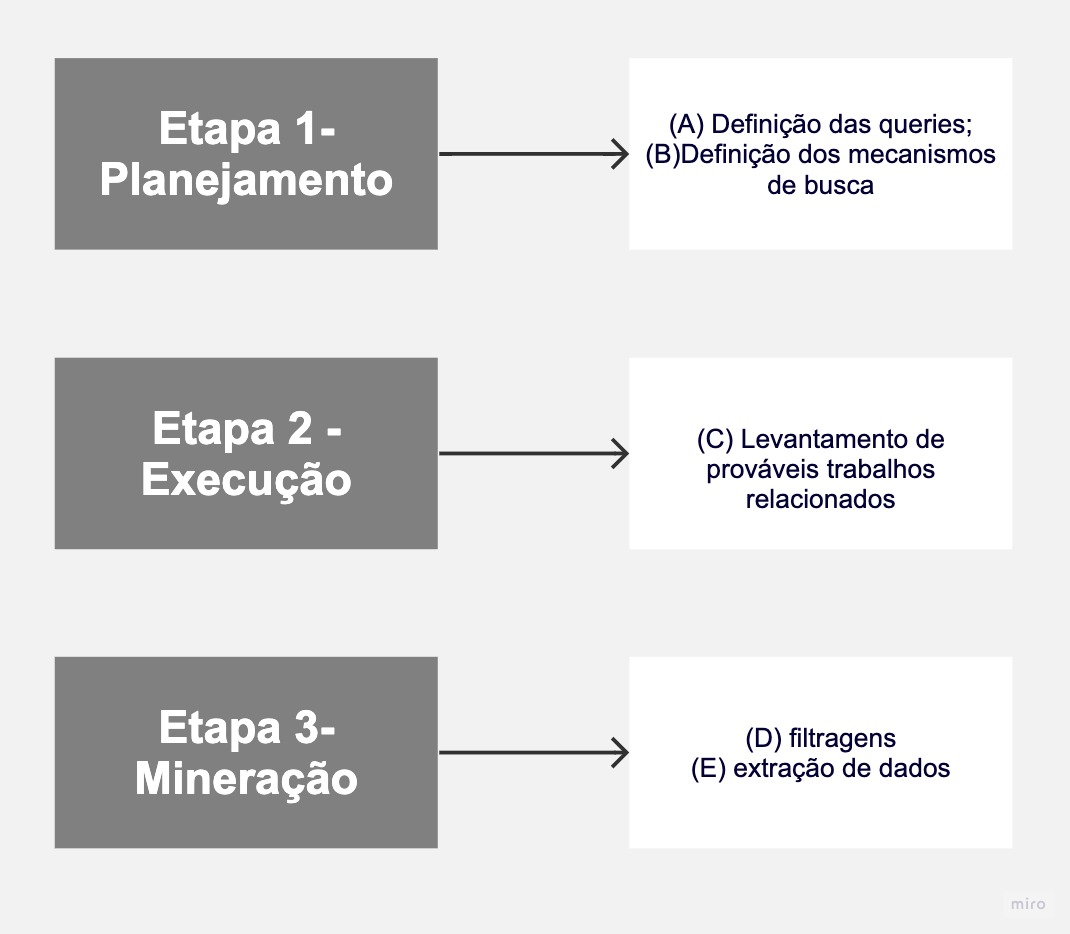
\includegraphics[width=8cm,height=\textwidth,keepaspectratio]{2-images/Fluxograma-artigos.jpg}
\newline \centering{Fonte: Elaborado pelo autor}\label{fig:processo_rev_sistematica}
\end{figure}


Detalham-se as etapas ilustradas na Figura \ref{fig:processo_rev_sistematica} conforme segue:

\begin{enumerate}
    
    \item As \textit{queries} são \textit{strings} que definem a lógica para seleção dos artigos. Para a presente pesquisa procurou-se buscar artigos cujo título ou \textit{keywords} contivessem as palavras \textit{AIOPs} além de limitar o intervalo de idade da publicação entre o ano de 2018 ao ano de 2023. Importante destacar que para o ano de 2023 foram considerados os seis primeiros meses.
    
    \item Por conhecida relevância na área da Ciência da Computação e, em especial, na área de Redes de Computadores, monitoramento e observabilidade, duas bases de pesquisa científica foram consideradas para execução das \textit{queries} em seus respectivos motores de busca: IEEExplore\footnote{https://ieeexplore.ieee.org/} e ACM \textit{Digital Library}\footnote{https://dl.acm.org/}.
    
    \item Após execução das \textit{queries} nas bases de pesquisa supracitadas foram obtidos 80 artigos. Uma distribuição da quantidade de artigos obtidos por ano de publicação pode ser observada na Figura \ref{fig:grafico_num_papers}:
      \begin{figure}[H]
    \centering
    \caption{Distribuição dos artigos obtidos pelo ano de publicação.} 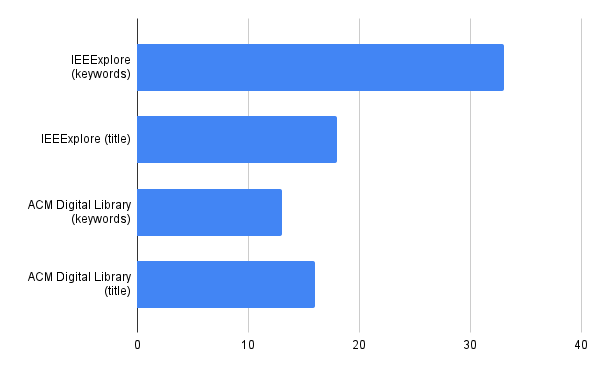
\includegraphics[width=12cm,height=\textwidth,keepaspectratio]{2-images/artigos-bars-horizontal.png}
    \newline \centering{ Fonte: Elaborado pelo autor}\label{fig:grafico_num_papers}
    \end{figure}
    \item A etapa de filtragem consistiu em eliminar artigos duplicados ou inacessíveis (22 em duplicidade e 2 sem acesso), e, posteriormente, realizou-se a leitura dos 56 artigos restantes onde observou-se que 35 não tinham relação direta com a linha de pesquisa objetivada nesta Dissertação de Mestrado. Portanto, após a aplicação dos filtros, 21 artigos foram identificados como fortemente relacionados ao tema objeto. A Figura \ref{fig:grafico_processamento_papers} resume a corrente etapa:
    
        \begin{figure}[H]
    \centering
    \caption{Detalhamento do resultado após os processos de filtragem dos artigos.} 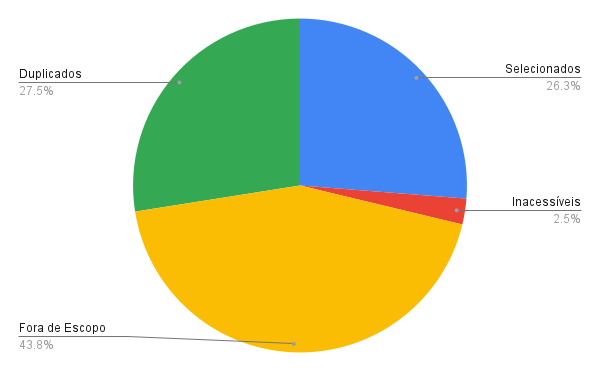
\includegraphics[width=10cm,height=\textwidth,keepaspectratio]{2-images/chart-2.png}
    \newline \centering{ Fonte: Elaborado pelo autor}\label{fig:grafico_processamento_papers}
    \end{figure}    

    \item Por fim, a quinta etapa consistiu na extração dos dados mais relevantes dos artigos selecionados. Foram extraídos para fins de observação de tendências as seguintes informações:
     \begin{itemize}
         \item Tipo de modelo: quais as técnicas de machine learning foram utilizadas ou sugeridas;
         \item \textit{Dataset}: quais as bases de dados usadas para realização dos testes;
         \item Arquitetura: quais arquiteturas proposta;
         \item \textit{Feature selection}: quais  \textit{features} foram utilizadas;
         \item Resultados: a quais resultados os autores chegaram, como RMSE e MAE; e
         \item Metodologia: quais materiais foram usados no processo de criação do modelo de  identificação de anomalias e predição (linguagens e softwares).
     \end{itemize}

\end{enumerate}

Os artigos selecionados são resumidos de forma a destacar os elementos mais importantes para relacionamento com a presente pesquisa. Os estudos foram organizados seguindo o seguinte critério:

\begin{itemize}
    \item Detalhamento dos trabalhos correlatos para o ano de 2018 na Subseção \ref{trab_correlatos_18};
    
    \item Detalhamento dos trabalhos correlatos para o ano de 2019 na Subseção \ref{trab_correlatos_19};
    
    \item Detalhamento dos trabalhos correlatos para o ano de 2020 na Subseção \ref{trab_correlatos_20};
    
    \item Detalhamento dos trabalhos correlatos para o ano de 2021 na Subseção \ref{trab_correlatos_21};
    
    \item Detalhamento dos trabalhos correlatos para o ano de 2022 na Subseção \ref{trab_correlatos_22};
    
    \item Detalhamento dos trabalhos correlatos para o ano de 2023 na Subseção \ref{trab_correlatos_23};
    
    
\end{itemize}

Para ilustrar todo o processo de Revisão Sistemática da Literatura, desde os detalhes das \textit{queries} até a extração dos dados mais relevantes, a Figura \ref{fig:diagrama_detalhado_rev_sistematica} exibe um fluxograma completo do processo utilizado:

\begin{figure}[H]
\centering
\caption{Fluxo detalhado do procedimento realizado na Revisão Sistemática da Literatura. } 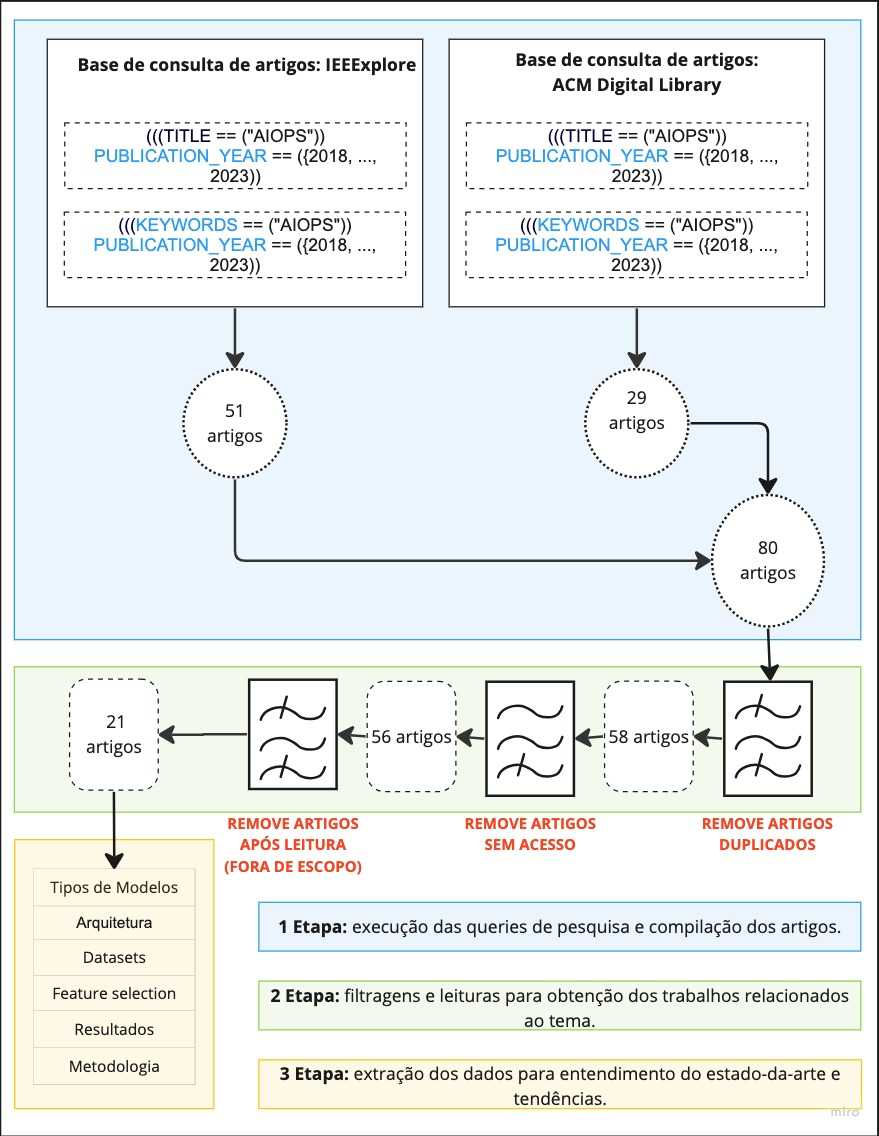
\includegraphics[width=\textwidth,keepaspectratio]{2-images/Fluxograma-papers.png}
\newline \centering{Fonte: Elaborado pelo autor}\label{fig:diagrama_detalhado_rev_sistematica}
\end{figure}    
    
    

\subsection{Trabalhos Correlatos - ano de 2018}\label{trab_correlatos_18}
Não foram encontrados trabalhos neste período.

\subsection{Trabalhos Correlatos - ano de 2019}\label{trab_correlatos_19}

Os autores \cite{8752866}, discutem no artigo (\textit{Anomaly Detection and Classification using Distributed Tracing and Deep Learning}) , a aplicação de Inteligência Artificial (IA) nas Operações de TI \textit{(AIOps)} para detectar anomalias com base em registros de \textit{distributed trancing}, que contêm informações detalhadas sobre a disponibilidade e o tempo de resposta dos serviços. Os autores propõem a detecção de anomalias no tempo de resposta, com aprendizado não supervisionado, baseada em técnicas de modelagem de dados de aprendizado profundo, e avalia a precisão e o desempenho da abordagem tanto em um ambiente de teste experimental quanto em uma nuvem em ambiente de produção em grande escala. Eles também mencionam as vantagens de combinar \textit{GRUs} (Unidades Recorrentes de Memória) e \textit{autoencoders} variacionais para aprender múltiplas distribuições complexas de dados em séries temporais geradas por sistemas de rastreamento distribuído.


\subsection{Trabalhos Correlatos - ano de 2020}\label{trab_correlatos_20}


Os autores \cite{9156101} ,  abordam o problema de monitoramento de um ambiente de TI complexo, incluindo nuvens privadas e públicas, ambientes de IoT, aplicativos e contêineres. A necessidade de um modelo de contexto nas Operações de TI é demonstrada para gerenciar as enormes quantidades de dados, armazenados em vários tipos de formatos e fornecer uma visão holística do ambiente de TI. A arquitetura proposta por eles trata-se de um \textit{framework} composto por cinco camadas: aquisição, gerenciamento, análise, apresentação de dados e respostas automatizadas. O \textit{Monitoring Resource Model} \textit{(MRM)} está no centro desse \textit{framework} e suporta a aquisição, o gerenciamento e a análise de dados de contexto, bem como uma camada de ação para fins de alerta e automação. Para isso, é proposto um modelo de aprendizado de máquina de redes neurais, o\textit{ Long-Short-Term-Memory (LSTM)}. Esses modelos são empregados para aprendizado supervisionado, a fim de prever o comportamento futuro dos sistemas monitorados.


\cite{9311349} Explicam sobre como a correlação, aprendizado de máquina e análise de big data podem reduzir o número de incidentes em infraestruturas de TI convergentes. O estudo enfatiza a importância do uso de técnicas de aprendizado de máquina, especialmente no contexto de (AIOps), para descobrir relacionamentos entre objetos e processos, e identificar padrões e sequências em milhões de eventos. A arquitetura proposta envolve a utilização de análise e aprendizado de máquina para investigar grandes quantidades de dados acumulados por diversos instrumentos e dispositivos de TI. Eles também mencionam a necessidade de dados de treinamento inicial representativos e pesquisas adicionais para melhorar as operações de TI em infraestruturas convergentes.

O objetivo do estudo apresendado por \cite{9443765}, é propor uma rede neural dinâmica, para prever fluxos de dados de séries temporais em cenários de AIOps, adim de realizar a previsão de tendência em tempo real de fluxos de dados. Os modelos de aprendizado de máquina utilizados incluem \textit{MWNN (Multi-Way Neural Network), WNN (Wavelet Neural Network) e LSTM (Long Short-Term Memory) }. Os dados utilizados durante os testes incluem conjuntos de dados de CPUs com diferentes capacidade. Os resultados obtidos mostram uma comparação com o consumo de recursos para MWNN, WNN e LSTM quando alcançam o mesmo desempenho, medido pela métrica RMSE. Também são fornecidos valores específicos de MSE, RMSE e MAE para os algoritmos nos mesmos dataset de CPUs .



\subsection{Trabalhos Correlatos - ano de 2021}\label{trab_correlatos_21}

Em seu estudo, os autores \cite{9516546} propõem a combinação de métodos integrados múltiplos para prever a capacidade de recursos. O modelo de aprendizado de máquina base utilizado é LSTM (Long Short-Term Memory). Usando o resultado desse modelo de previsão integrado com base nos dados históricos,  o estudou mostrou resultados interessantes no \textit{forecast} de recursos de TI, como o uso de CPU, disco rígido, memória. Isso pode ajudar a otimizar a capacidade de gerenciar os recursos  para manter o sistema estável e confiável. 


\cite{9605403} discutem o conceito de Machine Reasoning (MR) e seu papel na melhoria das Operações de Inteligência Artificial (AIOps) para Redes Baseadas em Intenções. MR é um ramo da Inteligência Artificial (IA) que se baseia na captura do conhecimento humano usando linguagens semânticas para mecanizar e executar fluxos de trabalho com um Motor de Raciocínio de Máquina (MRE). Eles mostram como esta abordagem complementa a Aprendizagem de Máquina (ML) fornecendo  precisão para inferências baseadas no conhecimento capturado e é adequado para resolver problemas que exigem profundo conhecimento de domínio. O cenário de uso porposto pelos autores, incluem MR em AIOps para automatizar e melhorar o processo de identificação da causa raiz de problemas em rede de computadores.

%27
\cite{9678534} Propõem um método chamado AID (Aggregated Intensity of Dependency), para prever de forma eficiente a intensidade de dependências em sistemas em nuvem em larga escala. O cenário utilizado pelos autores, envolve medir a intensidade de dependências em um sistema em nuvem de produção utilizando modelo de aprendizado de máquina. Durante os testes apresentado, dois conjuntos de dados foram utilizados: um conjunto de dados simulados gerados a partir de um sistema de microsserviços de referência e um conjunto de dados industriais coletados de um sistema em nuvem de produção. Os resultados da avaliação experimental mostraram que o método proposto mede com precisão a intensidade das dependências e supera várias bases de comparação.


%31
No artigo abordado pelos autores \cite{9680514}, é mostrado o design e a implementação de recursos para migrar os dados de sistemas de monitoramento antigos de uma aplicação nativa em nuvem para instâncias do Prometheus com \textit{framework Ananke}, e permitir a integração das séries temporais armazenadas no Prometheus com ferramentas padrão disponíveis em bibliotecas Python para análise de dados . O estudo também propõe uma estratégia de dimensionamento automático com base na previsão de picos de tráfego para uma aplicação web usando o modelo Facebook Prophet. O cenário de uso envolveu monitorar e modelar aplicações nativas de nuvem, com foco em métricas de desempenho de aplicativos reaia e estratégias de otimização envolvendo big data e AI/ML em  feedback contínuo . Em relação aos dados utilizados nos testes, os autores fizeram uso das séries temporais do Prometheus com métricas de servidores web como \textit{wordpress} coletados pelos mesmos.


\subsection{Trabalhos Correlatos - ano de 2022}\label{trab_correlatos_22}

%34
\cite{9492267} apresentam o TSAGen, uma ferramenta de geração de séries temporais, que pode ser usada para gerar dados sintéticos, fornecendo uma fonte de dados confiável para os demais pesquisadores. O TSAGen permite que os usuários avaliem de forma abrangente o desempenho de algoritmos de detecção de anomalias com dados sintéticos. A ferramenta aborda desafios como gerar anomalias diversas, ajustar a gravidade das anomalias e controlar as características dos KPIs gerados. A arquitetura proposta do TSAGen segue um design modular aditivo, em que cada componente é gerado independentemente para permitir simples integração de módulos individuais adicionais, de acordo com o cenário de cada pesquisa ou algoritmo.

%36
No estudo proposto pelos autores \cite{9746242}, é proposto uma rede neural profunda, chamada CDX-Net, para previsão de séries temporais multivariadas, no campo de Inteligência Artificial para Operações de TI (AIOps). O caso de uso envolve a modelagem e análise de dados de monitoramento, que são frequentemente representados como Séries Temporais Multivariadas (MTS). A arquitetura proposta do CDX-Net inclui módulos como ASPP, SRM, CAM, GRU, transformador e AB, que visam melhorar os procedimentos de extração e fusão de características. Os pesquisadores utilizam em seus experimentos, um conjunto de dados de uma aplicação web e compara o desempenho do modelo proposto com outros métodos de referência para Time Series.


%37
\cite{9746416} apresentam uma solução para o Desafio ICASSP-SPGC-2022 AIOps, uma competição organizada pela universidaade de \textit{Honk Kong}, mais especificamente para inferência precisa de combinações em \textit{root cause analysis}. O documento descreve os desafios nos dados da competição e propõe uma estrutura para resolver o problema. A arquitetura proposta inclui um método para inferir se uma amostra inclui múltiplas causas-raiz e a introdução de \textit{TextCNN}. O artigo também menciona que o método obteve uma pontuação de 0,93 e ficou em 4º lugar no \textit{leaderboard}.


%38
O estudo dos autores \cite{9789784}, propõe um método para gerar relatórios de falhas legíveis por humanos em sistemas de TIC, aproveitando dados de séries temporais e metadados textuais de métricas, a fim de detectar falhas em um sistema-alvo. É utilizado modelo LSTM (Long Short-Term Memory) para séries temporais multivariadas, que serve como o método de referência para comparação. A arquitetura proposta utiliza dados de séries temporais e metadados como entrada e gera um relatório de falha em formato de texto. Durante os testes, os autores utilizaram conjuntos de dados coletados de um sistema de microsserviços implantado em um cluster Kubernetes, os experimentos avaliaram a eficácia e o desempenho do método proposto na detecção de falhas em comparação com o método de referência. Os resultados experimentais mostraram que o método proposto alcançou alta precisão na detecção de cenários específicos, como consumo excessivo de CPU, vazamento de memória, e dados de rede.


%40
\cite{9825776} propõem uma representação gráfica para o DevOps em aplicações baseadas em aprendizado de máquina, também conhecida como MLOps, eles discutem a fase de planejamento do MLOps, onde o problema a ser resolvido e os dados disponíveis são identificados, abordagens de análise de dados adequadas e algoritmos são selecionados. Também mencionam a fase de codificação, onde o sistema e o código de ML são implementados e validados, e a fase de validação, que envolve a avaliação do desempenho do modelo de ML com novos dados. O artigo destaca a necessidade de um processo de MLOps integrado e menciona desafios na adoção do MLOps na prática.

%41
\cite{9835411} sugerem um \textit{framework} de dimensionamento automático proativo chamado RobustScaler para o cenário de computação em nuvem. O objetivo deste estudo é desenvolver um framework de dimensionamento automático que possa gerar decisões de mudança e elasticidade, otimizando o equilíbrio entre custo e Qualidade de Serviço (QoS), e que seja robusto a ruídos, dados ausentes e anomalias.  O modelo proposto captura tanto a periodicidade quanto a estocasticidade das chegadas de consultas e é treinado usando um algoritmo de Método dos Multiplicadores de Direção Alternada (ADMM). A arquitetura proposta do framework consiste em quatro componentes principais: detecção de periodicidade, modelagem histórica de chegadas de consultas, previsão de chegada de consultas e plano de dimensionamento 

%43
Neste artigo, os autores \cite{9892264}, apresentam um framework baseado em aprendizado federado chamado EFL-WP para previsão de carga de trabalho em ambientes de inter-nuvem. O framework proposto tem como objetivo colaborar para treinar modelos de machine learning para previsão de carga de trabalho sem compartilhar informações sensiveis. Para isso os autores sugerem p uso de modelos LSTM para prever a utilização da CPU, utilização de memória e outras métricas de desempenho. A arquitetura proposta consiste em um coordenador e treinadores, onde o coordenador agenda tarefas de treinamento, orquestra os treinadores e mantém modelos globais, enquanto os treinadores usam seus próprios dados para treinar modelos locais .


%45
\cite{9978983} abordam um método chamado "PUTraceAD" Positive-Unlabeled ,para  detecção de anomalias em \textit{tracing} de microsserviços . A arquitetura proposta envolve três etapas: Embedding de Span, Construção de Grafo de Rastros e Treinamento do Modelo, utilizando uma GNN (Graph Neural Network) e aprendizado PU para detectar anomalias em trancing. O conjunto de dados usado para os experimentos é chamado de TrainTicket, um sistema de referência de microsserviços, e os experimentos foram realizados em um cluster Kubernetes. Os resultados dos experimentos avaliam a eficácia e eficiência do PUTraceAD, bem como o impacto de diferentes configurações ,

%46
Neste artigo, os autores\cite{9985105} discutem sobre o Sistema de Gerenciamento de Dependências ou em inglês, Dependency Management System (DMS), para gerenciar dependências de serviços em sistemas em nuvem. O DMS é uma plataforma de ponta a ponta que oferece suporte completo ao ciclo de vida para garantir a confiabilidade do serviço, incluindo implantação inicial, atualização , otimização arquitetural pró-ativa e mitigação reativa de falhas. Os dados usados nos testes do DMS incluem informações de dependência coletadas de trancing distribuído, arquivos de configuração, consultas do orquestrador de serviços e relatórios de dependência de implantação.


%47
Com base nas questões relacionadas à implementação da observabilidade em sistemas de informações hospitalares (HIS) os autores \cite{10004053} abordam uma arquitetura de microsserviços e AIOps (Inteligência Artificial para Operações de TI). De forma contextual, o artigo faz pesquisa literária e apresenta um resumo de conceitos relacionados, incluindo as definições de observabilidade e HIS, requisitos e ideias de solução de observabilidade em cenários específicos, além de responder a perguntas pré-propostas. A arquitetura proposta envolve a aplicação de microsserviços e AIOps para alcançar a observabilidade do HIS, sendo fatores-chave indicadores como qualidade e escala de dados. O documento também fornece sugestões para o departamento de TI do hospital sobre como lidar com essas questões. 

%48
\cite{10020986} abordam uma análise de AIOps (Inteligência Artificial para Operações de TI) na gestão unificada de resiliência de dados em data lakehouses. O artigo propõe soluções para prever violações de Recovery Point Objective  (RPO) e fornecer sugestões aos SREs (Engenheiros de Confiabilidade do Site) sobre como configurar recursos do sistema para evitar violações de RPO. O artigo utiliza aprendizado supervisionado em conjunto com análise de séries temporais e propõe um modelo de aprendizado de máquina com uso de métodos combinados de aprendizado online e offline e filtragem de solicitações previstas para filtrar solicitações futuras estáveis.


\subsection{Trabalhos Correlatos - ano de 2023}\label{trab_correlatos_23}


%56
\cite{10098585} os autores fornecem informações sobre a implementação de baselines usando Python e regressão linear como o modelo de aprendizado de máquina, as questões de pesquisa e o design experimental, a aplicação na análise de desempenho, distribuições de latência, o uso de cargas de trabalho continuamente variáveis e a configuração experimental.

%57
\cite{10113794} abordam o desenvolvimento de um sistema de detecção de outlier chamado OutSpot para datacentes com alto nivel de desempenho e alta criticidade, que basicamente atuam com o fornecimento de streaming de videos. O sistema tem como objetivo detectar outliers nos KPIs coletados desses datacenters.  O modelo de ML utilizado, integra Hierarchical Agglomerative Clustering (HAC), com Conditional Variational Autoencoder (CVAE). O HAC é aplicado para agrupar os KPIs com base em seus padrões, e as informações de agrupamento de cada KPI são, então incorporadas ao método CVAE. Essa abordagem permite que o OutSpot detecte outliers para KPIs em larga escala com padrões diversos A arquitetura proposta do OutSpot envolve dividir os conjuntos de dados coletados em conjuntos de treinamento e teste. O conjunto de treinamento consiste em dados dos primeiros 7 dias, enquanto o conjunto de teste é composto por dados do último dia. O conjunto de teste é rotulado por operadores experientes usando uma ferramenta desenvolvida pelos autores. Os outliers são rotulados por três operadores, sendo a decisão final tomada quando seus rótulos divergem.
